\begin{tikzpicture}[x=1cm,y=1cm]
  \fill[infPaper] (-0.30,-17.05) rectangle (25.45,0.20);

  % COL 1: INSTRUCCIONISMO VS ECONOMIA DEL CONOCIMIENTO
  \draw[fill=white,draw=infGreen,line width=1.1pt,rounded corners=7pt] (0.0,-15.72) rectangle (8.15,0.0);
  \fill[infGreen,rounded corners=6pt] (0.0,-2.48) rectangle (8.15,0.0);
  \fill[infGreen] (0.0,-2.48) rectangle (8.15,-2.00);
  \node[anchor=north west,text width=5.45cm,align=left,inner sep=0pt] at (0.28,-0.22) {%
    {\color{white}\fontsize{11.5}{13.5}\selectfont\bfseries Keith Sawyer (I)\par}\vspace{2pt}%
    {\color{white!90}\fontsize{7.3}{8.6}\selectfont\bfseries Crisis del instruccionismo\\y economía creativa\par}\vspace{3pt}%
    {\colorbox{infGreenAccent}{\color{white}\fontsize{6.3}{7.3}\selectfont\bfseries\ Eje 1 · Modelo Estándar vs. Siglo XXI \ }}%
  };
  \node[inner sep=0pt] at (6.92,-1.24) {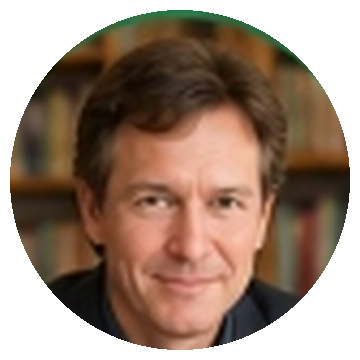
\includegraphics[width=2.06cm]{img_infografia/sawyer_photo.png}};

  \fill[infGreenLight] (0.12,-3.04) rectangle (8.03,-2.56);
  \node[font=\fontsize{6.9}{8.0}\selectfont\bfseries\color{infGreen}] at (4.075,-2.80) {Mejorando el aprendizaje: ciencias del aprendizaje (2008)};

  \InfSectionBar{0.20}{-3.16}{infGreen}{infGreenLight}{target}{Idea central del eje}
  \node[anchor=north west,text width=7.65cm,align=left,font=\fontsize{6.6}{8.0}\selectfont\color{infInk},inner sep=0pt] at (0.25,-3.74) {%
    La escuela fabril surgió sin investigación empírica sobre cómo aprendemos; hoy la economía creativa requiere «analistas simbólicos» capaces de modelar, innovar y transferir ideas.%
  };

  \InfSectionBar{0.20}{-4.86}{infGreen}{infGreenLight}{key}{Conceptos clave}
  \InfConceptCard{0.20}{-5.44}{infGreen}{infGreenCard}{alerta}{\textbf{Instruccionismo}\\Transmisión lineal fabril (Papert).}
  \InfConceptCard{2.17}{-5.44}{infGreen}{infGreenCard}{cerebro}{\textbf{Analista simbólico}\\Creación e ingenio conceptual.}
  \InfConceptCard{4.14}{-5.44}{infGreen}{infGreenCard}{escuela}{\textbf{Saber situado}\\Sujeto, herramientas y contexto.}
  \InfConceptCard{6.11}{-5.44}{infGreen}{infGreenCard}{construccion}{\textbf{Práctica experta}\\Participar en quehacer científico.}

  \InfSectionBar{0.20}{-7.78}{infGreen}{infGreenLight}{bulb}{Aportes principales}
  \InfBullet{0.22}{-8.38}{infGreen}{Supuesto tradicional: conocer es acumular hechos sueltos y procedimientos cuya ordenación definieron adultos.}
  \InfBullet{0.22}{-9.04}{infGreen}{Las ciencias del aprendizaje unen psicología cognitiva, computación, neurociencias, sociología y diseño.}
  \InfBullet{0.22}{-9.70}{infGreen}{El conocimiento no es estructura estática dentro del cráneo: emerge en actividad social situada.}
  \InfBullet{0.22}{-10.36}{infGreen}{Formar técnicos e ingenieros exige practicar modelos y explicaciones auténticas, no memoria repetitiva.}

  \InfSectionBar{0.20}{-11.12}{infGreen}{infGreenLight}{gear}{Implicaciones en Matemáticas}
  \InfCheck{0.22}{-11.72}{infGreen}{Sustituir series repetitivas por desafíos de modelación real.}
  \InfCheck{0.22}{-12.26}{infGreen}{Conectar variables simbólicas con mediciones de taller.}
  \InfCheck{0.22}{-12.80}{infGreen}{Reconocer límites de aplicación física de cada fórmula.}
  \InfCheck{0.22}{-13.34}{infGreen}{Actuar el aula como laboratorio interdisciplinario activo.}

  \fill[infGreenLight,rounded corners=5pt] (0.20,-15.52) rectangle (7.95,-14.05);
  \node[text width=7.35cm,align=center,font=\fontsize{6.6}{8.1}\selectfont\color{infGreen}] at (4.075,-14.78) {%
    \textbf{\textit{«El modelo estándar preparó para la fábrica, pero limita la comprensión profunda hoy necesaria.»}}\\
    {\scriptsize — Eje histórico · Sawyer (2008)}%
  };

  % COL 2: HALLAZGOS COGNITIVOS, ARTICULACION Y ANDAMIAJE
  \draw[fill=white,draw=infNavy,line width=1.1pt,rounded corners=7pt] (8.50,-15.72) rectangle (16.65,0.0);
  \fill[infNavy,rounded corners=6pt] (8.50,-2.48) rectangle (16.65,0.0);
  \fill[infNavy] (8.50,-2.48) rectangle (16.65,-2.00);
  \node[anchor=north west,text width=5.45cm,align=left,inner sep=0pt] at (8.78,-0.22) {%
    {\color{white}\fontsize{11.5}{13.5}\selectfont\bfseries Keith Sawyer (II)\par}\vspace{2pt}%
    {\color{white!90}\fontsize{7.3}{8.6}\selectfont\bfseries Hallazgos cognitivos,\\articulación y andamiaje\par}\vspace{3pt}%
    {\colorbox{infBlueAccent}{\color{white}\fontsize{6.3}{7.3}\selectfont\bfseries\ Eje 2 · Mecanismos del Aprendizaje \ }}%
  };
  \node[inner sep=0pt] at (15.42,-1.24) {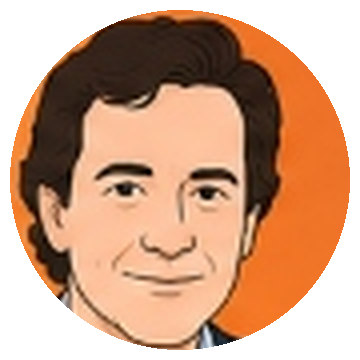
\includegraphics[width=2.06cm]{img_infografia/sawyer_illus.png}};

  \fill[infBlueLight] (8.62,-3.04) rectangle (16.53,-2.56);
  \node[font=\fontsize{6.9}{8.0}\selectfont\bfseries\color{infNavy}] at (12.575,-2.80) {Saberes previos, pensamiento visible y scaffolding efectivo};

  \InfSectionBar{8.70}{-3.16}{infNavy}{infBlueLight}{target}{Idea central del eje}
  \node[anchor=north west,text width=7.65cm,align=left,font=\fontsize{6.6}{8.0}\selectfont\color{infInk},inner sep=0pt] at (8.75,-3.74) {%
    Comprender profundamente ocurre al integrar hechos en redes conceptuales, explicitar «matemáticas ingenuas», externalizar razonamientos en voz alta y graduar el andamiaje docente.%
  };

  \InfSectionBar{8.70}{-4.86}{infNavy}{infBlueLight}{key}{Conceptos clave}
  \InfConceptCard{8.70}{-5.44}{infNavy}{infBlueCard}{lupa}{\textbf{Ideas ingenuas}\\Teorías previas del aprendiz.}
  \InfConceptCard{10.67}{-5.44}{infNavy}{infBlueCard}{dialogo}{\textbf{Articulación}\\Pensar en voz alta y explicar.}
  \InfConceptCard{12.64}{-5.44}{infNavy}{infBlueCard}{target}{\textbf{Metacognición}\\Monitorear el propio camino.}
  \InfConceptCard{14.61}{-5.44}{infNavy}{infBlueCard}{andamio}{\textbf{Andamiaje}\\Guía que se retira con autonomía.}

  \InfSectionBar{8.70}{-7.78}{infNavy}{infBlueLight}{bulb}{Aportes principales}
  \InfBullet{8.72}{-8.38}{infNavy}{Los aprendices no llegan como vasos vacíos: su error suele expresar una teoría intuitiva coherente que debe aflorar.}
  \InfBullet{8.72}{-9.04}{infNavy}{La pericia experta combina esquemas ricos, adaptación improvisada en el espacio del problema y reflexión.}
  \InfBullet{8.72}{-9.70}{infNavy}{Articulación y comprensión se refuerzan mutuamente: explicar a otros acelera el dominio conceptual.}
  \InfBullet{8.72}{-10.36}{infNavy}{El buen andamiaje da pistas y preguntas detonadoras sin resolver la tarea en lugar del estudiante.}

  \InfSectionBar{8.70}{-11.12}{infNavy}{infBlueLight}{gear}{Implicaciones en Matemáticas}
  \InfCheck{8.72}{-11.72}{infNavy}{Diagnosticar confusión entre $y=kx$ e $y=mx+b$ antes de operar.}
  \InfCheck{8.72}{-12.26}{infNavy}{Exigir justificaciones escritas de pendiente y ordenada inicial.}
  \InfCheck{8.72}{-12.80}{infNavy}{Retirar apoyos en tablas guía conforme progresa el bloque.}
  \InfCheck{8.72}{-13.34}{infNavy}{Incorporar diarios breves de reflexión metacognitiva al cierre.}

  \fill[infBlueLight,rounded corners=5pt] (8.70,-15.52) rectangle (16.45,-14.05);
  \node[text width=7.35cm,align=center,font=\fontsize{6.6}{8.1}\selectfont\color{infNavy}] at (12.575,-14.78) {%
    \textbf{\textit{«Decir cómo hacer todo ayuda en lo inmediato, pero anula el andamiaje que construye autonomía.»}}\\
    {\scriptsize — Eje cognitivo · Sawyer (2008)}%
  };

  % COL 3: DISENO DE AMBIENTES, TIMSS Y EVALUACION
  \draw[fill=white,draw=infOrange,line width=1.1pt,rounded corners=7pt] (17.00,-15.72) rectangle (25.15,0.0);
  \fill[infOrange,rounded corners=6pt] (17.00,-2.48) rectangle (25.15,0.0);
  \fill[infOrange] (17.00,-2.48) rectangle (25.15,-2.00);
  \node[anchor=north west,text width=5.45cm,align=left,inner sep=0pt] at (17.28,-0.22) {%
    {\color{white}\fontsize{11.5}{13.5}\selectfont\bfseries Keith Sawyer (III)\par}\vspace{2pt}%
    {\color{white!90}\fontsize{7.3}{8.6}\selectfont\bfseries Diseño de ambientes, TIMSS\\y evaluación profunda\par}\vspace{3pt}%
    {\colorbox{infOrangeAccent}{\color{white}\fontsize{6.3}{7.3}\selectfont\bfseries\ Eje 3 · Principios de Rediseño Escolar \ }}%
  };
  \node[inner sep=0pt] at (23.92,-1.24) {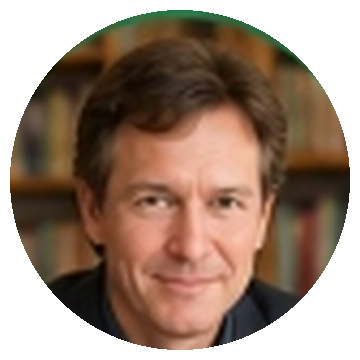
\includegraphics[width=2.06cm]{img_infografia/sawyer_photo.png}};

  \fill[infOrangeLight] (17.12,-3.04) rectangle (25.03,-2.56);
  \node[font=\fontsize{6.9}{8.0}\selectfont\bfseries\color{infOrange}] at (21.075,-2.80) {Personalización, conocimiento distribuido y lección TIMSS};

  \InfSectionBar{17.20}{-3.16}{infOrange}{infOrangeLight}{target}{Idea central del eje}
  \node[anchor=north west,text width=7.65cm,align=left,font=\fontsize{6.6}{8.0}\selectfont\color{infInk},inner sep=0pt] at (17.25,-3.74) {%
    Un aula rediseñada combina fuentes plurales, personalización sensible, colaboración intelectual, menor saturación temática y evaluación centrada en comprensión conceptual integrada.%
  };

  \InfSectionBar{17.20}{-4.86}{infOrange}{infOrangeLight}{key}{Conceptos clave}
  \InfConceptCard{17.20}{-5.44}{infOrange}{infOrangeCard}{personas}{\textbf{Saber distribuido}\\Equipos y herramientas reales.}
  \InfConceptCard{19.17}{-5.44}{infOrange}{infOrangeCard}{grafica}{\textbf{Lección TIMSS}\\Coherencia supera cobertura.}
  \InfConceptCard{21.14}{-5.44}{infOrange}{infOrangeCard}{doc}{\textbf{Evaluación real}\\Medir integración y sentido.}
  \InfConceptCard{23.11}{-5.44}{infOrange}{infOrangeCard}{balanza}{\textbf{Rol profesional}\\Docente diseñador y tutor.}

  \InfSectionBar{17.20}{-7.78}{infOrange}{infOrangeLight}{bulb}{Aportes principales}
  \InfBullet{17.22}{-8.38}{infOrange}{Estudios TIMSS prueban que planes saturados de temas superficiales logran menor desempeño matemático.}
  \InfBullet{17.22}{-9.04}{infOrange}{El maestro deja de ser única fuente de saber; coordina libros, simuladores, expertos y trabajo tutelado.}
  \InfBullet{17.22}{-9.70}{infOrange}{Las pruebas estandarizadas convencionales ignoran errores conceptuales profundos y desincentivan el proyecto.}
  \InfBullet{17.22}{-10.36}{infOrange}{Conectar escuela, museos, aprendizaje tutelado (\textit{apprenticeship}) y formación continua supera fronteras rígidas.}

  \InfSectionBar{17.20}{-11.12}{infOrange}{infOrangeLight}{gear}{Implicaciones en Matemáticas}
  \InfCheck{17.22}{-11.72}{infOrange}{Priorizar pocas familias de modelos estudiadas a profundidad.}
  \InfCheck{17.22}{-12.26}{infOrange}{Valorar coherencia entre tabla, gráfica, ecuación y texto.}
  \InfCheck{17.22}{-12.80}{infOrange}{Evaluar dictámenes técnicos por fases con retroalimentación.}
  \InfCheck{17.22}{-13.34}{infOrange}{Articular la autonomía del profesorado técnico en academia.}

  \fill[infOrangeLight,rounded corners=5pt] (17.20,-15.52) rectangle (24.95,-14.05);
  \node[text width=7.35cm,align=center,font=\fontsize{6.6}{8.1}\selectfont\color{infOrange}] at (21.075,-14.78) {%
    \textbf{\textit{«El profesorado debe actuar como trabajador del conocimiento, igual que médicos o ingenieros.»}}\\
    {\scriptsize — Eje sistémico · Sawyer (2008)}%
  };

  % PIE DE FUENTE Y CREDITOS
  \draw[fill=infGreen,draw=infGreen,rounded corners=6pt] (0.0,-16.92) rectangle (25.15,-15.88);
  \node[inner sep=0pt] at (0.72,-16.40) {\InfIconOutline[0.36]{libro}{white}};
  \node[anchor=west,text width=16.8cm,align=left,font=\fontsize{6.6}{8.0}\selectfont\color{white}] at (1.30,-16.40) {%
    \textbf{FUENTE BASE (APA 7):} Sawyer, R. K. (2008). Optimizing learning: Implications of learning sciences research. En OECD/CERI, \textit{Innovating to learn, learning to innovate} (cap. 2, pp. 45--65). OECD Publishing. \url{https://doi.org/10.1787/9789264039958-en}%
  };
  \node[anchor=east,text width=6.4cm,align=right,font=\fontsize{6.1}{7.4}\selectfont\color{white!90}] at (24.90,-16.40) {%
    \textbf{Mtro. Martín Jonathan de la Cruz Muñoz (Matrícula 00874)}\\
    IIIEPE · MAEM · Fundamentos para la Enseñanza y el Aprendizaje I%
  };
\end{tikzpicture}